%% For double-blind review submission
\documentclass[sigplan,10pt,review]{acmart}
\settopmatter{printfolios=true}
%% For final camera-ready submission
%\documentclass[acmlarge]{acmart}\settopmatter{}

\makeatletter\if@ACM@journal\makeatother

%% Journal information (used by PACMPL format)
%% Supplied to authors by publisher for camera-ready submission
\acmJournal{PACMPL}
\acmVolume{1}
\acmNumber{1}
\acmArticle{1}
\acmYear{2017}
\acmMonth{1}
\acmDOI{10.1145/nnnnnnn.nnnnnnn}
\startPage{1}
\else\makeatother

%% Conference information (used by SIGPLAN proceedings format)
%% Supplied to authors by publisher for camera-ready submission
\acmConference[PL'17]{IEEE}{2018}{Planet Earh}
\acmYear{2017}
\acmISBN{978-x-xxxx-xxxx-x/YY/MM}
\acmDOI{10.1145/nnnnnnn.nnnnnnn}
\startPage{1}
\fi

\newcommand{\fer}[1]{\textcolor{red}{#1}}

%% For review submission
\setcopyright{none}

%% Bibliography style
\bibliographystyle{ACM-Reference-Format}
%\citestyle{acmauthoryear}

%% Packages that we are using in this version of the work:
\usepackage{amsmath}
\usepackage{hyperref}
\usepackage{paralist}
\usepackage[brazil]{babel}
\usepackage[utf8]{inputenc}
\usepackage{mathpartir}


% To turn comments OFF simply comment out the \Commentstrue line
\newif\ifComments\Commentstrue

\ifComments
\newcommand{\marcio}[1]{\noindent\textcolor{violet}{Marcio: {#1}}}
\newcommand{\guido}[1]{\noindent\textcolor{magenta}{Guido: {#1}}}
\newcommand{\fernando}[1]{\noindent\textcolor{brown}{Fernando: {#1}}}
\newcommand{\cesar}[1]{\noindent\textcolor{magenta}{Cesar: {#1}}}
\newcommand{\pedro}[1]{\noindent\textcolor{brown}{Pedro: {#1}}}
\newcommand{\rmv}[1]{\noindent\textcolor{gray}{Removed: {#1}}}
\newcommand{\new}[1]{\noindent\textcolor{blue}{ {#1}}}
\newcommand{\ed}[1]{\noindent\textcolor{red}{ {#1}}}
\else
\newcommand{\marcio}[1]{}
\newcommand{\guido}[1]{}
\newcommand{\fernando}[1]{}
\newcommand{\cesar}[1]{}
\newcommand{\pedro}[1]{}
\newcommand{\rmv}[1]{}
\newcommand{\new}[1]{#1}
\newcommand{\ed}[1]{}
\fi
\newcommand\dawn{\mbox{\textsf{DawnCC}}}
\newcommand\Taskminer{\mbox{\textsf{TaskMiner}}}

\newtheorem{Challenge}{Challenge}[section]

\begin{document}

\title[Automatic Identification and Annotation of Tasks in Structured
Programs]
{TaskMiner: Identificação Automática de Tarefas}

\author{Pedro Henrique Ramos Costa}
\authornote{with author1 note}          %% \authornote is optional;
\orcid{nnnn-nnnn-nnnn-nnnn}
\affiliation{
  \position{Researcher}
  \department{DCC}
  \institution{UFMG}
  \streetaddress{6627 Antonio Carlos Avenue}
  \city{Belo Horizonte}
  \state{Minas Gerais}
  \postcode{31.270-213}
  \country{Brazil}
}
\email{pedroramos@dcc.ufmg.br}

\author{Gleison Souza Diniz Mendonc\c{c}a}
\authornote{with author1 note}          %% \authornote is optional;
\orcid{nnnn-nnnn-nnnn-nnnn}
\affiliation{
  \position{Researcher}
  \department{DCC}
  \institution{UFMG}
  \streetaddress{6627 Antonio Carlos Avenue}
  \city{Belo Horizonte}
  \state{Minas Gerais}
  \postcode{31.270-213}
  \country{Brazil}
}
\email{gleison.mendonca@dcc.ufmg.br}

\author{Guilherme Mendes Leobas}
\authornote{with author1 note}          %% \authornote is optional;
\orcid{nnnn-nnnn-nnnn-nnnn}
\affiliation{
  \position{Researcher}
  \department{DCC}
  \institution{UFMG}
  \streetaddress{6627 Antonio Carlos Avenue}
  \city{Belo Horizonte}
  \state{Minas Gerais}
  \postcode{31.270-213}
  \country{Brazil}
}
\email{guihermel@dcc.ufmg.br}

\author{Fernando M Q Pereira}
\authornote{with author1 note}
\orcid{nnnn-nnnn-nnnn-nnnn}
\affiliation{
  \position{Professor}
  \department{DCC}
  \institution{UFMG}
  \streetaddress{6627 Antonio Carlos Avenue}
  \city{Belo Horizonte}
  \state{Minas Gerais}
  \postcode{31.270-213}
  \country{Brazil}
}
\email{fernando@dcc.ufmg.br}          %% \email is recommended

\begin{abstract}
Este artigo apresenta \Taskminer{}, uma ferramenta capaz de encontrar paralelismo de tarefas
em código C automaticamente. \Taskminer{} lida com problemas clássicos de paralelismo irregular como
encontrar os limites simbólicos de acesso à memória em tempo de execução, remoção de dependências
estáticas espúrias, contornar condições de corrida ao transformar código sequencial em código paralelo, e
principalmente, encontrar o equilíbrio entre tamanho de uma tarefa e excesso de paralelismo, em contraste com
o custo de manutenção de tarefas pelo ambiente de execução. Para contornar esses problemas,
\Taskminer{} implementa uma série de otimizações e análises em representação intermediária do LLVM, resultando
em um compilador fonte-a-fonte capaz de analisar código C e inserir no mesmo anotações OpenMP automaticamente. \Taskminer{} prova-se eficaz ao encontrar paralelismo apontado manualmente em benchmarks como \textsf{BSC-Bots}~\cite{Duran09}, produzindo programas tão rápidos ou mais velozes que as versões sequenciais e anotadas manualmente, além de encontrar paralelismo escondido em programas sequenciais, absolutamente sem intervenção humana.
\end{abstract}

%% 2012 ACM Computing Classification System (CSS) concepts
%% Generate at 'http://dl.acm.org/ccs/ccs.cfm'.
 \begin{CCSXML}
<ccs2012>
<concept>
<concept_id>10010147.10010169.10010175</concept_id>
<concept_desc>Computing methodologies~Parallel programming languages</concept_desc>
<concept_significance>500</concept_significance>
</concept>
<concept>
<concept_id>10010147.10011777.10011014</concept_id>
<concept_desc>Computing methodologies~Concurrent programming languages</concept_desc>
<concept_significance>500</concept_significance>
</concept>
<concept>
<concept_id>10011007.10011006.10011041</concept_id>
<concept_desc>Software and its engineering~Compilers</concept_desc>
<concept_significance>500</concept_significance>
</concept>
</ccs2012>
\end{CCSXML}

\ccsdesc[500]{Computing methodologies~Parallel programming languages}
\ccsdesc[500]{Computing methodologies~Concurrent programming languages}
\ccsdesc[500]{Software and its engineering~Compilers}

\keywords{Parallelism, Tasks, OpenMP}

\maketitle

\section{Introdu\c{c}\~{a}o}
\label{sec:intro}

É inegável que computação paralela e distribuída é hoje a alternativa mais procurada por 
desenvolvedores em sua busca por desempenho. Programadores tem cada vez mais investido
em paradigmas paralelos, visando maior eficiência e velocidade. Nesse contexto, sistemas de
anotação como OpenMP~\cite{JaegerCP15},
OpenACC~\cite{OpenACC20}, OpenHMPP~\cite{Andion14}, OpenMPC~\cite{Lee10},
OpenSs~\cite{MeenderinckJ11}, Cilk++~\cite{Leiserson09} e
OmpSs~\cite{bueno:icpp:2011, duran:ppl:2011}
atuam como metalinguagem, conferindo ao programador
poder semântico para transformar um programa originalmente sequencial
em um programa paralelo. Tais sistemas mostram-se muito promissores quando
combinados com aceleradores como GPUs e FPGAs~\cite{Bertolli14,Martineau16,Mendonca17,Poesia17,Reyes12,Antao16,Wienke12}.
Entretanto, apesar de conveniente, o uso desses sistemas não é automático e
requer exaustiva escrutinação de olho humano para garantia de corretude e eficiência.

Embora já existam ferramentas que inserem anotações automaticamente 
em programas~\cite{Amini12,Guelton12,Mendonca16,Pingali11,Nugteren14},
todas essas tecnologias exploram somente paralelismo de dados.  Porém, grande
parte do poder de sistemas de anotação provém da capacidade de se criar \textit{tarefas}
durante a execução do programa~\cite{Ayguade09}. Dessa forma, o propósito desse trabalho
é apresentar um algoritmo capaz de minerar oportunidades para paralelismo de tarefas
em programas sequênciais e anotá-los automaticamente. Como descrito na seção \ref{sec:ovf},
essas anotações conferem ao programa irregular semântica de algoritmos em grafos e/ou \textit{worklists}~\cite{Ben-Nun17,Kulkarni11,Pingali11}.

O presente artigo descreve {\Taskminer}, um compilador fonte-a-fonte que expõe
paralelismo de tarefas em programas C/C++. {\Taskminer} lida com diversos desafios 
do universo do paralelismo irregular. Primeiro, deve-se determinar os limites
simbólicos dos blocos de memória acessados dentro de cada programa. Depois,
encontra-se regiões ou fragmentos de código (laços ou funções) que podem 
ser efetivamente mapeados à tarefas. Então, deve-se extrair parâmetros capazes
de estimar o custo da tarefa em questão. Esses parâmetros estão dinamicamente atrelados
às anotações e são capazes de ativar ou desativar a criação de tarefas durante a execução do programa,
ou de limitar a profundidade de tarefas geradas recursivamente. Após feito isso, deve-se determinar
quais variáveis serão privatizadas em novas tarefas, ou compartilhadas por tarefas concorrentes.
Finalmente, deve-se mapear todas essas informações de volta ao código fonte, produzindo
anotações legíveis.

Este trabalho defende a tese de que a anotação automática de tarefas é útil à medida que
retira do programador o fardo de procurar, anotar e verificar as anotações, tornando seu
processo de desenvolvimento mais eficiente. A ferramenta {\Taskminer} é capaz
de alcançar ganhos de quase 4x em benchmarks não usualmente paralelos, como descrito em \ref{sec:eval}. {\Taskminer}
recebe como input um programa escrito em C e produz como output um programa também em C,
mas anotado com diretivas OpenMP legíveis. {\Taskminer} anota programas não triviais, envolvendo
todo tipo de construto da linguagem C como arranjos, estruturas, uniões e ponteiros para esses tipos.
Alguns desses programas provém de benchmarks complexos como Kastor~\cite{Virouleau14}, Bots~\cite{Duran09}  e a suíte de testes do LLVM~\cite{Lattner04}.
As versões anotadas pelo {\Taskminer} se aproximam das versões anotadas manualmente em
desempenho, e são mais rápidos que as versões sequenciais.


\section{Visão geral}
\label{sec:ovf}

A construção de um compilador como o \Taskminer{} envolve a superação de uma série de etapas e desafios.
\Taskminer{} recebe como entrada um programa escrito em C e retorna o mesmo programa anotado com 
diretivas OpenMP. Como descrito por LaGrone et al. ~\cite{LaGrone11}, 
o ambiente de execução OpenMP se encarrega de 
rastrear dependências entre ponteiros estaticamente. Entretanto, a inserção
automática das anotações é apenas a última etapa. Nesta Seção detalharemos os desafios e problemas
encontrados pelo \Taskminer{} no processo de mineração de tarefas. A solução para esses problemas será descrita 
posteriormente na Seção~\ref{sec:sol}.

\begin{figure}[b!]
\begin{center}
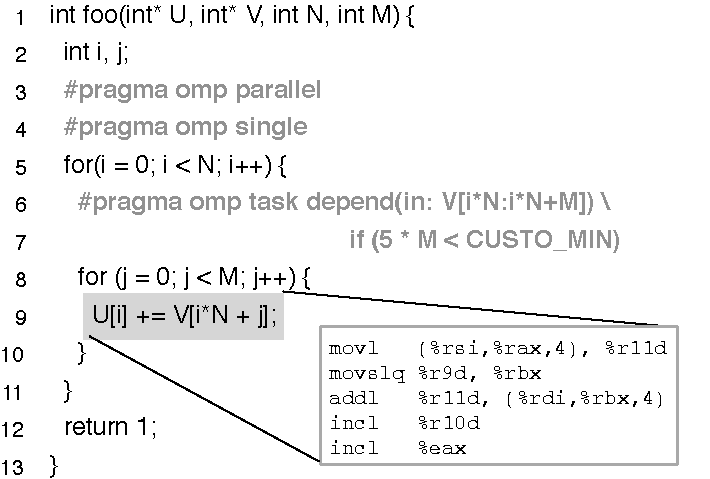
\includegraphics[width=1\columnwidth]{images/ex_Regions}
\caption{Identificando limites de memória e o custo de uma tarefa.}
\label{fig:ex_Regions}
\end{center}
\end{figure}

O primeiro desafio encontrado pelo \Taskminer{} consiste em 
identificar regiões de memória cobertas por uma tarefa.
A Figura~\ref{fig:ex_Regions} ilustra esse problema e como resolvê-lo. Este programa recebe
uma matriz $\mathsf{M}\times\mathsf{N}$ identificada por  \textsf{V}, em formato linear,
e produz um vetor  \textsf{U} de forma que  \textsf{U[i]} contenha a soma de todos
os elementos na linha  \textsf{i} da matriz  \textsf{V}. {\Taskminer} determina que cada
iteração do laço mais externo pode se tornar uma tarefa. Então, cada tarefa neste programa
consiste no laço mais interno, e atravessa a região de memória entre os endereços  \textsf{\&V + i * N} e
 \textsf{\&V + i * N + M}. A identificação desses limites envolve o uso de álgebra simbólica baseada
 na literatura de compiladores.
 
A Figura~\ref{fig:ex_Regions} também apresenta um outro problema: {\em como estimar a rentabilidade de uma tarefa?}
A criação de tarefas envolve um custo alto por parte do ambiente de execução, causado por questões como
alocação, escalonamento, concorrência e gerenciamento em tempo real do grafo de dependências de tarefas.
Idealmente, são desejáveis tarefas que executem uma quantidade de trabalho
grande o suficiente para superar este custo. Como consta em \cite{Rice53}, a quantidade de trabalho executado
por uma tarefa não pode ser descoberta estaticamente. É possível aproximar-se dessa quantia utilizando-se
símbolos nativos do programa, que, em execução, serão substituídos por valores. 
Por exemplo, na figura~\ref{fig:ex_Regions}
é conhecido o número de instruções do laço interno. Então aproxima-se a quantidade de trabalho executado
com a expressão \textsf{5 * M}. Dessa forma, o valor de \textsf{M} durante a execução será determinante para
a criação da tarefa. Essa checagem é feita na linha 7 da Figura, 
e faz parte da sintaxe de OpenMP. Além disso, {\Taskminer} propõe
uma estimativa confiável a respeito do limite mínimo de custo 
que uma tarefa deve possuir para ser criada sem produzir
excesso de computação. Esse limite considera fatores como número de 
núcleos disponíveis e informações a respeito do ambiente
de execução em termos de instruções de máquina.
	
\begin{figure}[h!]
\begin{center}
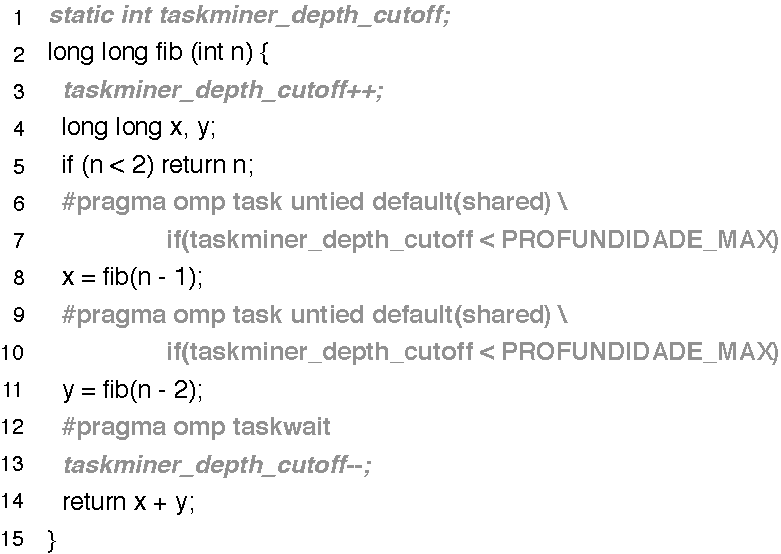
\includegraphics[width=1\columnwidth]{images/ex_cutoff}
\caption{limitando a criação de tarefas recursivas.
Exemplo retirado de~\cite[Fig.1]{Iwasaki16}.}
\label{fig:ex_cutoff}
\end{center}
\end{figure}
	
No paralelismo de tarefas, um fator importante para bom desempenho
é o uso de cortes mínimos para o número de tarefas a serem criadas~\cite{Duran08b}. 
Observa-se esse fator explicitamente no contexto de tarefas recursivas. 
Para limitar a criação de tais tarefas, que tem uma granularidade menor,
uma variável de controle é inserida no código. 
Um exemplo é ilustrado na Figura~\ref{fig:ex_cutoff}. 
Um contador é associado à invocação de funções recursivas anotadas com diretiva de tarefas. 
A checagem na linha 7 certifica-se de que o limite
nunca é excedido. Esse limite é pré-determinado na fase de configuração do 
{\Taskminer}, assim como o limite de trabalho mínimo
por tarefa. Dessa forma, observa-se que a geração 
de código executada pelo {\Taskminer} é dependente de dois parâmetros,
\textsf{DEPTH\_CUTOFF} e \textsf{WORK\_CUTOFF}. 
Eles possuem valores por padrão, mas podem ser configurados pelo usuário.

\begin{figure}[h!]
\begin{center}
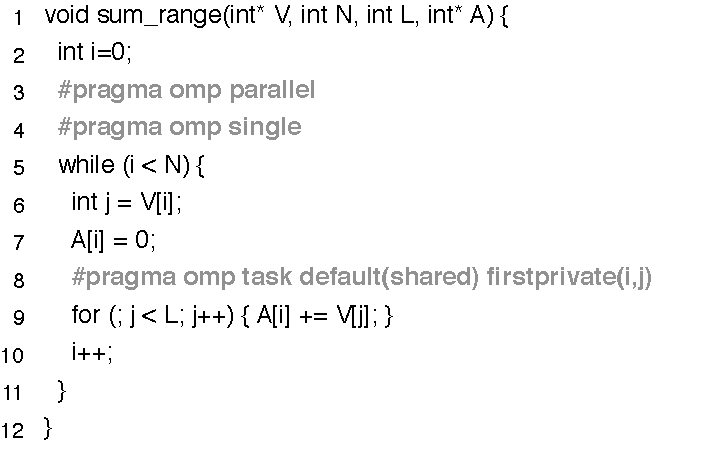
\includegraphics[width=1\columnwidth]{images/ex_privatize}
\caption{A variável \textsf{j} deve ser replicada em todas as tarefas para evitar condições de corrida.}
\label{fig:ex_privatize}
\end{center}
\end{figure}

Por fim,  um último problema surge ao transformar um programa originalmente
sequencial em um programa paralelo. Condições de corrida evidenciam
quais variáveis devem ser replicadas e
quais podem ser compartilhadas pelas tarefas. 
Assim como o problema de determinar os limites de acesso à memória, 
se não resolvido, esse problema pode levar à programas incorretos.
Esse processo de replicação de variáveis em todas as tarefas criadas se chama \textit{privatização}. 
Na Figura~\ref{fig:ex_privatize}, por exemplo,
a variávei \textsf{j} deve ser privatizada. 
Caso não seja, ela será compartilhada por todas as tarefas 
criadas na linha 5 da Figura~\ref{fig:ex_privatize}. 
{\Taskminer} utiliza uma técnica descrita na seção~\ref{sec:sol} 
para resolver esse problema.	

\section{Solu\c{c}\~{a}o}
\label{sec:sol}

\begin{figure}[b]
\begin{center}
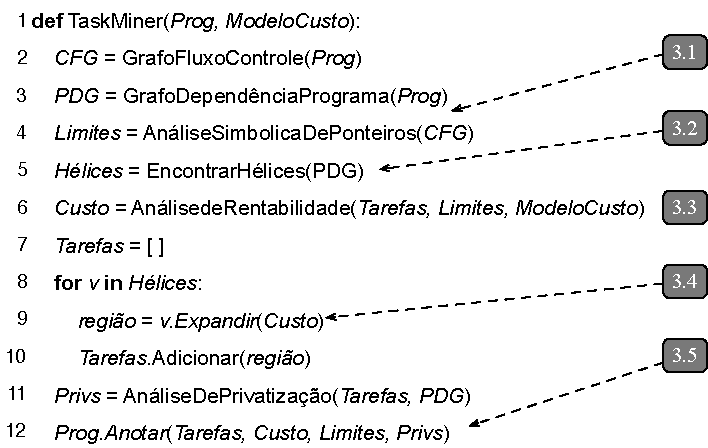
\includegraphics[width=1\columnwidth]{images/alg_main}
\caption{Os principais passos do algoritmo do TaskMiner.}
\label{fig:alg_main}
\end{center}
\end{figure}

A figura~\ref{fig:alg_main} descreve o algoritmo executado pela ferramenta {\Taskminer}. Ele utiliza conceitos conhecidos como
o grafo de dependências~\cite{Ferrante87} e o grafo de fluxo de controle~\cite{Kildall73}. O objetivo principal do {\Taskminer}
é identificar tarefas em programas estruturados. Programas estruturados podem ser particionados em regiões \textit{hammock}
\cite{Ferrante87}.

\begin{definition} [Região \textit{Hammock}]
\label{def:hammock}
Um grafo de fluxo de controle $G$ é um grafo direcionado com um nó de entrada
$s$ e um nó de saída $x$. Uma região \textit{hammock} $G'$ é um subgrafo de $G$ com um nó $h$ que {em domina}
\footnote{Um nó $n_1 \in G$ domina outro nó
$n_2 \in G$ de todo caminho de  $S$ até $n_2$ atravessa $n_1$.
Inversamente, $n_1$ pós-domina $n_2$ se todo caminho de $n_2$ até $x$ deve passar por $n_1$.} os outros nós em $G$.
Além disso, existe um nó $w \in G$, $w \notin G'$, tal que $w$ {\em pós-domina} todo nó em $G'$. Nessa definição,
$h$ é o nó de entrada e $w$ é o nó de saída de $G'$.  
\end{definition}

\begin{definition} [Tarefa]
\label{def:task}
Dado um programa $P$, uma tarefa $T$ é uma tupla $(G', M_i, M_o)$ formada
por uma região \textit{hammock} $G'$ e um conjunto $M_i$ de dependências de memória representando
os dados lidos por $T$ e um conjunto $M_o$ de regiões de memória que representam dados escritos por $T$.
\end{definition}

Sintaticamente, regiões de memória são descritas por variáveis do programa e/ou ponteiros com intervalos derefenciáveis.
Dadas duas tarefas $T_1 = (G_1, M_{i1}, M_{o1})$ e $T_2 = (G_2, M_{i2}, M_{o2})$, 
se $M_{o1} \cap M_{i2} \neq \emptyset$ então $T_2$ {\em depende} de $T_1$. Se um programa $P$ está particionado em um 
conjunto de $n$ tarefas, então ele deve respeitar a Definição \ref{def:corretude} para ser considerado correto:

\begin{definition} [Corretude]
\label{def:corretude}
Um conjunto $T$ de $n$ tarefas é uma paralelização correta de um programa $P$ se:
\begin{compactenum}
\item $T$ não contém dependências cíclicas;
\item A execução das tarefas em $T$ em qualquer ordem determinada pelas relações de dependência devem resultar
identicamente à execução sequencial de $P$.
\end{compactenum}
\end{definition}

Abaixo há um exemplo de como as regiões de memória são marcadas em uma anotação de tarefa.
Considere-se duas tarefas $T_{\mathit{foo}} = (\mathsf{foo}, \{\mathsf{v[i - 1]}\},
\{v[i]\})$ e $T_{\mathit{bar}} = (\mathsf{bar}, \{v[i]\}, \{\})$. Dependências são identificadas na cláusula \textit{depend}. 
Nesse exemplo, cada região \textit{hammock} é constituída por uma chamada de função:

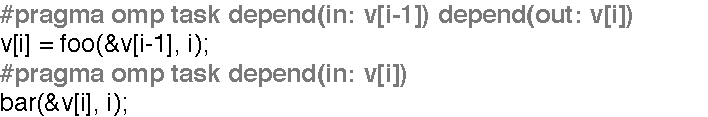
\includegraphics[width=1\columnwidth]{images/ex_depends}

{\Taskminer} utiliza OpenMP 4.0 para explorar o paralelismo de tarefas. Detalhes da sintaxe e semântica
das anotações do OpenMP estão publicamente disponíveis\footnote{``Summary of OpenMP 4.0 C/C++ Syntax", disponibilizado
pelo grupo OpenMP}. As anotações utilizadas são:
%
\begin{compactitem}
\item \textsf{parallel}: compõe um time de \textit{threads}
para executar uma região do programa marcada como paralela.
\item \textsf{single}: especifica uma região que deve ser executada
por apenas uma \textit{thread} do time.
\item \textsf{task}: cria uma nova tarefa.
\item \textsf{taskwait}: define um ponto de sincronização para aquela
região paralela.
\end{compactitem}
%
Algumas dessas anotações são associadas a uma lista de cláusulas, a seguir:
\begin{compactitem}
\item \textsf{default([shared/private])}: indica que a variável é compartilhada ou replicada
entre tarefas.
\item \textsf{firstprivate($v$)}: indica que $v$ deve ser replicada entre tarefas e inicializada
com o valor corrente no ponto de execução da anotação.
\item \textsf{untied}: indica que uma tarefa não está associada firmemente à uma única \textit{thread},
permitindo ao ambiente balancemanto e preempção.
\item \textsf{depend}($\mathit{in}/\mathit{out}/\mathit{inout}$): determina se um dado é lido, escrito
ou ambos, efetivamente estabelecendo as dependências entre as tarefas.
\item \textsf{if}({\em condição}): define uma condição para que aquela anotação seja executada.
\end{compactitem}

\subsection{Encontrando limites simbólicos}
\label{sec:sra}

Para produzir uma anotação que criará uma tarefa $T = (G, M_i, M_o)$,
é necessário determinar as regiões de memória $M_i$ que $T$ lê, e as regiões
$M_o$ em que $T$ escreve. Para tal, recorre-se à análise de limites simbólicos.
 
 Por exemplo, a instrução \textsf{U[i] += V[i*N + j]}, na linha 9 da Figura~\ref{fig:ex_Regions}
 contém dois acessos à memória: \textsf{U[i]} e
\textsf{V[i*N + j]}.
 O primeiro cobre a região de memória $[\mathtt{\&}\mathsf{U},
\mathtt{\&}\mathsf{U} + (\mathsf{M} - 1) \times \mathsf{sizeof}(\mathtt{int})]$.
O segundo cobre a região 
$[\mathtt{\&}\mathsf{V} + \mathsf{N} \times \mathsf{sizeof}(\mathtt{int}), \mathtt{\&}\mathsf{V} + ((\mathsf{i} \times \mathsf{M} + j) - 1) \times \mathsf{sizeof}(\mathtt{int})]$.
Não há código na Figura~\ref{fig:ex_Regions} que dependa do laço nas linhas 8-10.
Portanto, uma anotação de tarefa deve considerar apenas a dependência de entrada, ou seja,
o acesso à \textsf{V}. É por isso que a cláusula \textsf{depend} na linha 6 contém uma referência
a essa região.

\begin{definition} [Análise de Limites Simbólicos]
\label{def:limites}
É uma forma abstrata de interpretação que associa uma variável inteira $v$
a um intervalo simbólico $R(v) = [l, u]$ em que $l$ e $u$ são expressões simbólicas.
Uma expressão simbólica $E$ é definida pela gramática abaixo, em que $s$ é um 
símbolo do programa:
\renewcommand{\arraystretch}{0.9}
\[
\begin{array}{rcl}
E & ::= & z \ \ | \ \ s \ \ | E + E \ \ | \ \ E \times E \ \ | \ \  \mbox{min}(E, E) \ \ | \\
&  & \mbox{max}(E, E) \ \ | -\infty \ \ | \ \ +\infty
\end{array}
\]
\end{definition}

Símbolos de programa são nomes que não podem ser construídos como funções de
outros nomes. Exemplos incluem variáveis globais, argumentos de função e valores retornados
por funções externas. Análise de limtes simbólicos não é uma contribuição deste artigo. A técnica
escolhida para as análises do {\Taskminer} é aquela implementada no compilador \dawn{} \cite{Mendonca17},
que, por sua vez, reusa trabalho de Blume {\em et al.}~\cite{Blume94}. Para este trabalho, é apenas
suficiente saber que essa implementação é sólida o suficiente para lidar com toda a linguagem C99, sempre termina
e executa em tempo quadrático no número de variáveis do programa, no pior caso.

Por exemplo, se aplicada à Figura~\ref{fig:ex_Regions}, a análise de limites resulta em 
$R(\mathsf{i}) = [0, \mathsf{N} - 1]$, e $R(\mathsf{j}) = [0, \mathsf{M} - 1]$.
O acesso à memória \textsf{V[i*N + j]} na linha 9, combinado a essa informação, fornece
a região simbólica que aparece na anotação da linha 6 na Figura~\ref{fig:ex_Regions}.

\subsection{Mapeando regiões em tarefas}
\label{sub:identification}

% Windmills and vanes
Uma {\em tarefa candidata} é um conjunto de instruções que podem executar paralelamente.
Para identificá-las, {\Taskminer} faz uso do {\em Grafo de Dependências}. 

\begin{definition} [Grafo de Dependências]~\cite{Ferrante87}
\label{def:pdg}
Dado um programa
$P$, seu PDG contém um vértice para cada instrução $s \in P$. Existe uma aresta de 
$s_1$ a $s_2$ se o último depende do primeiro. $s_2$ tem uma dependência de dados de $s_1$
se lê dados que $s_1$ escreve. $s_2$ tem uma dependência de controle de $s_1$ se $s_1$ controla
a execução de $s_2$ a partir do resultado de um \textit{branch}, por exemplo.
\end{definition}

Tarefas candidatas são \textbf{hélices em moinhos}. {\em Moinhos} são uma família de grafos ~\ref{Rideau08}.
Moinhos existem como subgrafos do grafo de dependências. 

\begin{definition} [Moinho]
\label{def:moinho}
Um moinho é um grafo $G_w = G_c \cup G_{v1} \cup \ldots \cup G_{vn}$
formado por componentes fortemente conexos $G_c$ (centro do Moinho) e $n$ componentes, não necessariamente
fortes, $G_{vi}$ chamados de hélices, tais que:
\begin{compactenum}
\item para qualquer ordenação topológica de $G_w$, e os nós $n_c \in G_c$,
$n_v \in G_{vi}$, $n_c$ está à frente de $n_v$;
\item para qualquer $i$ e $j$, $1 \leq i < j \leq n$, $G_{vi}$ e $G_{vj}$ não
compartilham vértices (portanto, compartilhar arestas também é impossível).
\end{compactenum}
\end{definition}

\begin{figure}[h]
\begin{center}
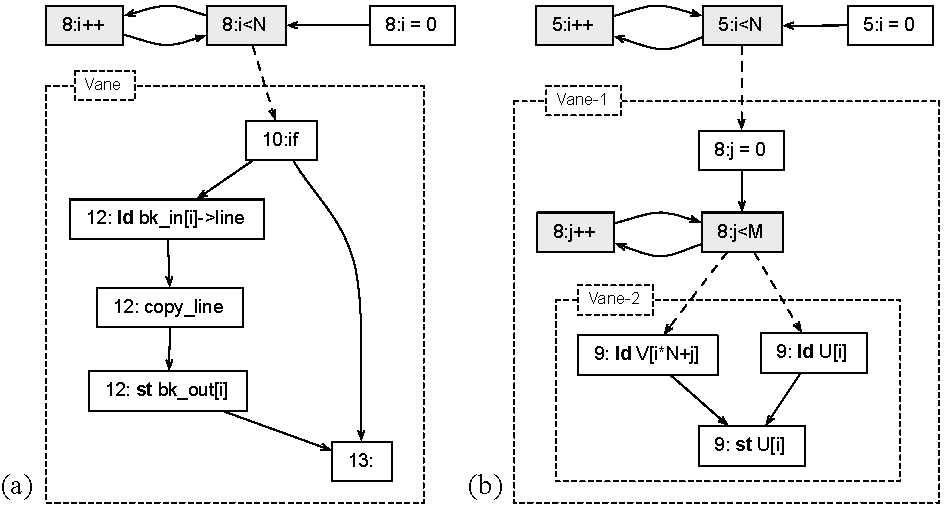
\includegraphics[width=1\columnwidth]{images/ex_windmill}
\caption{Exemplos de grafos de dependências. Nós que formam centros de moinhos
são coloridos de cinza. Arestas sólidas representam dependências de dados; arestas pontilhadas
dependências de controle. Hélices de moinhos aparecem dentro de retângulos pontilhados.
Na imagem, vemos o grafo para a Figura~\ref{fig:ex_Regions} em (b).}
\label{fig:ex_windmill}
\end{center}
\end{figure}

A Figura ~\ref{fig:ex_windmill} mostra dois grafos de dependências, bem como seus
moinhos e hélices. A estrutura de moinhos naturalmente evidencia tarefas candidatas.
Hélices correspondem à partes do programa que tem alta probabilidade de serem
executadas diversas vezes, pois surgem de um laço: o centro do moinho. Duas execuções
de uma mesma hélice podem ser paralelas. Esta é uma propriedade do grafo de dependências, e uma 
das motivações originais para este trabalho. Essas duas execuções podem ser vistas como duas instâncias
da mesma estrutura: a hélice, partindo do mesmo centro do moinho. Uma ordenação topológica desse grafo não impõe
nenhuma ordem entre essas duas hipotéticas réplicas de uma mesma hélice.

Moinhos contém propriedades estruturais para identificação de tarefas. Moinhos são encontrados
em uma simples busca em profundidade no grafo de dependências. Entretanto, nem todo moinho
evidencia tarefas proveitosas. Além disso, alguns moinhos não podem ser anotados devido à inabiliadde 
da análise de ponteiros em encontrar limites de acesso à memória. As próximas seções tratam desses
problemas.

\subsection{Estimando a lucratividade de tarefas}
\label{sub:profit}

O benefício de criar tarefas depende de dois fatores: custo de execução e paralelismo.
A dificuldade surge em encontrar o ponto mediano entre tarefas grandes demais e tarefas pequenas.
Tarefas muito pequenas tendem a ser mais paralelas, pois tendem a ter menos dependências. Entretanto,
se uma tarefa é muito pequena, então os ganhos de performance são eclipsados pelo custo do ambiente de execução
em manter essa tarefa ativa, e o paralelismo extra não compensa o custo de gerenciamento desta tarefa.
Por outro lado, se tarefas são muito grandes, então não há paralelismo: tarefas individuais executarão sequencialmente.
{\Taskminer} marca como tarefa aquelas hélices que são maximais em termos de custo de execução, ou seja, as menores hélices
que estão acima do custo de execução no ambiente escolhido.

O tamanho de uma tarefa é dado pelo número de instruções contidas na mesma. A mesma região de um programa
pode levar à criação de tarefas com tamanhos diferentes. Portanto, o tamanho real de uma tarefa só é conhecido ao final 
da execução da mesma. Entretanto, para julgar se acriação de uma tarefa vale a pena, é necessário aproximar esse tamanho
estaticamente. Com esse objetivo em mente, define-se a noção de {\em Trabalho Estatico Estimado}:

% Explain the tension between large and small tasks.
\begin{definition}[Trabalho Estático Estimado (TEE)]
\label{def:swe}
Seja $G = G_1 \cup G_2 \cup \ldots \cup G_n$ uma partição de um grafo de controle
de um $G$ em $n$ regiões hammock {\em disjuntas}.
Trabalho Estático Estimado ($W(G)$) é definido como um número real não negativo,
tal que $W(G) = W(G_1) + W(G_2) + \ldots + W(G_n)$.
\end{definition}

O objetivo é obter um $W$ próximo ao comportamento dinâmico dos programas.
A heurística mais conhecida na literatura para a proximação de $W$ é o 
\textit{profiler} estático implementado por Wu e Larus~\cite{Wu94}.
A heurística escolhida para este trabalho utiliza a análise de limites
descrita na Seção \ref{sub:sra} para inserir informações dinâmicas em ambiente estático,
através da construção de expressões simbólicas que representam o número de iterações
de laços, similar à técnica implantada para migração de memória virtual em arquiteturas NUMA
\cite{Piccoli14}. Essas expressões são inseridas em condicionais para a criação da
tarefa, como ilustrado na linha 7 da Figura \ref{fig:ex_Regions}.

\begin{figure}[t!]
\begin{small}
\begin{eqnarray*}
\begin{tabular}{lc}
\textsc{[Instr]} &
W(\mbox{instr}) = \mbox{given by the spec.}
\\\\
\textsc{[Seq]} &
\inferrule{W(S_1) = w_1 \\ W(S_2) = w_2}{W(S_1;S_2;) = w_1 + w_2}
\\\\
\textsc{[Branch]} &
\inferrule{W(S_1) = w_1 \\ W(S_2) = w_2 \\ W(S_3) = w_3}
{W(\mbox{if}(S_1) \ S_2; \ \mbox{else} \ S_3;) = w_1 + \mbox{max}(w_2, w_3)}
\\\\
\textsc{[LoopInf]} &
\inferrule{W(S_1) = w_1 \\ W(S_2) = w_2 \\ \mathit{Iter}(S_1) = \infty}
{W(\mbox{while} (S_1) \ S_2;) = 10 \times (w_1 + w_2)}
\\\\
\textsc{[LoopExp]} &
\inferrule{W(S_1) = w_1 \\ W(S_2) = w_2 \\ \mathit{Iter}(S_1) = E}
{W(\mbox{while} (S_1) \ S_2;) = E \times (w_1 + w_2)}
\end{tabular}
\end{eqnarray*}
\end{small}
\caption{\label{fig:swe}Estimando o custo das tarefas.}
\end{figure}

% Explain how we use symbolic information to compute costs.
As regras declarativas da Figura~\ref{fig:swe} esboçam as heurísticas
utilizadas para computar o TEE para uma região hammock $S$.
A regra \textsc{LoopInf} aplica-se a laços cujo número de iterações não
pode ser limitado por uma expressão simbólica computada estaticamente.
Assume-se que laços executam ao menos 10 vezes~\cite{Wu94}.
A regra \textsc{LoopExp} representa laços que não podem ser analisados 
com a análise de limites simbólicos. A função auxiliar $\mathit{Iter}(S)$ 
retorna uma expressão simbólica que representa a variedade de valores
cobertos pelo código em $S$ que controla o número de iterações do laço.
Essas regras são implementadas durante o passo de estimativa da lucratividade.

\paragraph{O Modelo de Custo.}
Um modelo de custo é uma coleção de parâmetros que determinam o impacto
da criação e manutenção de tarefas em uma determinada arquitetura.
A literatura lista técnicas analíticas~\cite{Baghsorkhi10} e empíricas~\cite{Poesia17}
para a construção do modelo. Um modelo de custo automático não é o objetivo deste trabalho.
Pelo contrário, o algoritmo do {\Taskminer} recebe um modelo de custo como parâmetro.
Para os experimentos descritos na Seção ~\ref{sec:eval}, utilizou-se constantes
relacionadas à criação de {\em threads} em uma determinada arquitetura. Por exemplo,
a criação de tarefas foi estimada em 500 ciclos para a arquitetura em que os experimentos
foram realizados.

% Discuss the expansion algorithm.
\subsection{Expansão de tarefas}
\label{sub:expansion}

Expansão de tarefas consiste em encontrar a menor tarefa que é grande o suficiente
para compensar o custo de criação de {\em threads}. A figura \ref{fig:expand_alg}
mostra o algoritmo de expansão. Inicia-se o algoritmo atribuindo \textsf{REGIÃO} a
um grafo hammock $H$ que corresponde a uma hélice em um moinho $W$.
A decomposição hammock de um programa estruturado forma uma árvore~\cite{Ferrante87},
em que os vértices representam grafos hammock.
$H_1$ é filho de $H_2$ na árvore se:
(i) $H_1 \subset H_2$, e (ii) para qualquer 
nó $H_x$, se $H_1 \subset H_x$ então $H_2 \subset H_x$.
Nese contexto, $H_2$ é {\em pai} de $H_1$.

\begin{figure}[h]
\begin{center}
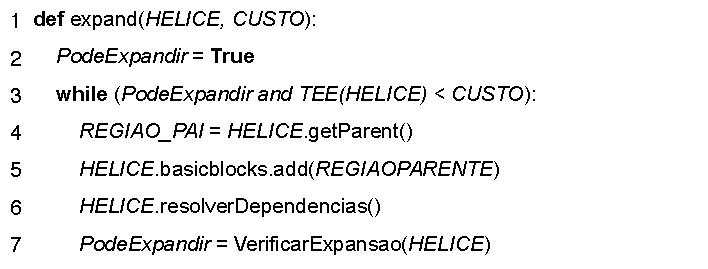
\includegraphics[width=1\columnwidth]{images/expand_alg}
\caption{Descoberta de tarefas em regiões hammock.
\textsf{CUSTO} é o custo de criação e escalonamento de {\em threads}.}
\label{fig:expand_alg}
\end{center}
\end{figure}

A cada nova expansão, checa-se se a expansão é válida. A expansão é válida se:
(i) \textsf{HÉLICE} está contida em um moinho $W$;
(ii) as regiões de memória em \textsf{HÉLICE} podem ser analisadas de acordo com
a seção \ref{sub:sra};
(iii) \textsf{HÉLICE} não depende de uma outra hélice no mesmo moinho $W$.

\begin{figure}[h]
\begin{center}
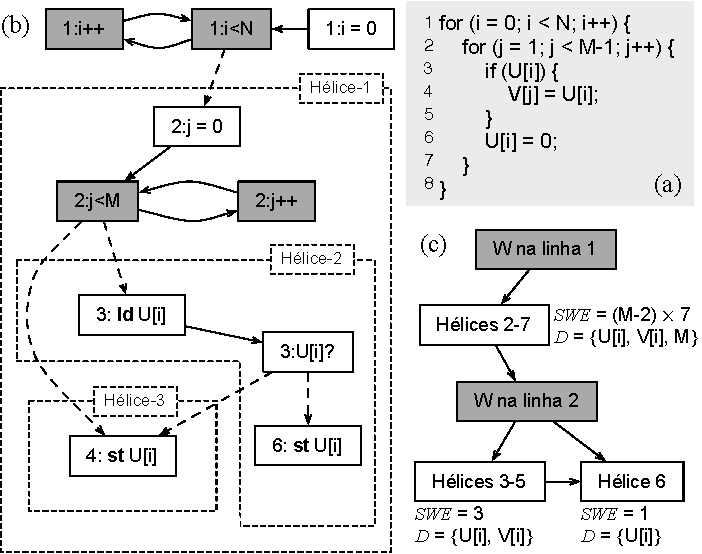
\includegraphics[width=1\columnwidth]{images/ex_expansion}
\caption{(a) Exemplo de laço duplamente aninhando analisado pelo {\Taskminer}.
(b) O Grafo de Dependências do programa.
(c) A decomposição desse laço em moinhos e hélices. $D$ é o conjunto de variáveis
das quais as hélices dependem.}
\label{fig:ex_expansion}
\end{center}
\end{figure}

O programa na Figura~\ref{fig:ex_expansion} (a) contém dois moinhos.
O primeiro consiste do laço da linha 1. O outro, aninhado, é o laço da linha 2.
As hélices que surgem desses moinhos estão evidenciadas na Figura~\ref{fig:ex_expansion} (b).
Na Figura, há 3 tarefas candidatas, cada uma formada por uma hélice diferente.
Para encontrar as tarefas, aplica-se a função de expansão (Fig.~\ref{fig:expand_alg})
nas hélices mais internas: \textsf{Hélice-2} pode ser expandida para incluir \textsf{Hélice-3}.

A expansão ocorre até o limite definido pelo \textsf{CUSTO}, que é determinado pelo modelo de custo
da Seção~\ref{sub:profit}. Se a lucratividade é menor que este custo, então
a criação da tarefa não é desejável. Porém, se a tarefa é expandida demais, 
há perda de paralelismo: o código executa sequencialmente. Portanto, determinar o \textsf{CUSTO}
é essencial para o desempenho do {\Taskminer}.

\subsection{Privatização de variáveis}
\label{sub:variance}

Para evitar condições de corrida, a inserção de anotações com semântica paralela
em programas sequenciais exige a replicação de alguns valores, tornando-os privados para cada tarefa.
Essa medida é chamada de {\em privatização}.

Se uma variável escalar contém pelo menos uma cadeia de definição-e-uso que entra
a fronteira de uma tarefa, então essa variável deve ser privatizada. A fronteira de uma 
tarefa é determinada pela função de expansão vista na Figura~\ref{fig:expand_alg}.

\begin{example}[Privatização]
\label{ex:priv}
Variáveis \textsf{i} e \textsf{j} na Figura~\ref{fig:ex_privatize} devem ser replicadas
nas tarefas indicadas pela anotação na linha 8.
A variável \textsf{i} é definida nas linhas 2 e 10, e utilizada na linha 9, que faz
parte do corpo de uma nova tarefa; \textsf{j} é definida na linha 6 e utilizada na linha 9.
Dessa forma, ambas possuem uma cadeia de definição-e-uso que ultrapassa a fronteira
de uma tarefa. Cada iteração do laço na linha 9 lê um valor diferente para \textsf{i}; portanto,
cada tarefa deve receber um valor diferente nesta variável. Na ausência de privatização, cada {\em thread}
leria o mesmo valor, de forma que a paralelização desse código o tornaria incorreto.
A privatização de \textsf{i} e\textsf{j} evita as condições de corrida e mantém o programa correto.
\end{example}

\subsection{Anotando o código fonte}
\label{sub:ir}

As análises descritas até agora foram implementadas na representação intermediária
do LLVM devido à facilidade do uso de análises como evolução escalar~\cite[p.18]{Grosser12} e outras
análises de fluxo de dados.
Porém, as anotações são inseridas em código fonte C, então grande
parte deste trabalho foi o mapeamento de informações da representação intermediária do LLVM de volta
para código C.

% Explain machinery: scope tree and simplification
\noindent
\textbf{Árvore de escopos:}
A árvore de escopos é uma estrutura utilizada pelo {\Taskminer} para mapear regiões hammock em construtos C, como blocos
\textsf{while} e \textsf{if-then-else}. Cada nó nesta árvore contém {\em meta-dados}
provenientes de informação de depuração obtida durante a compilação para representação
intermediária do LLVM. Para manter esse tipo de informação de depuração, basta compilar o código com a flag
{\em -g}.
É possível achar o número da linha relacionada à cada nó na árvore de escopos, permitindo
ao {\Taskminer} a anotação das regiões hammock no código fonte de maneira precisa.

\paragraph{Limitando a criação de tarefas recursivas}
Para evitar a criação excessiva de tarefas muito pequenas, {\Taskminer} concede a opção
aos usuários de limitar a criação de tarefas. Por exemplo \textsf{./Taskminer -r 12} limita o número
de tarefas criadas um total de 12 tarefas. Essa solução é implementada diretamente no código-fonte,
na fase final. Embora simples, conforme experimentos (Sec.~\ref{sec:eval}), essa solução traz claros
benefícios em benchmarks recursivos. A variável, chamada de \textsf{taskminer\_depht\_cutoff} na Figura
\ref{fig:ex_cutoff}, é global e ligada estaticamente no programa. No começo de cada função recursiva,
esta variável é incrementada para indicar a criação de uma nova tarefa; e decrementada ao sair da mesma função.

\begin{example}[Limitação de tarefas]
A Figura~\ref{fig:ex_cutoff} ilustra a estratégia utilizada pelo {\Taskminer} para limitar
o número de tarefas criadas durante a invocação de uma função recursiva.
O parâmetro \textsf{DEPHT\_CUTOFF} é determinado pelo usuário.
\end{example}

Há outras formas de limitar o número de tarefas recursivas~\cite{Iwasaki16,Iwasaki16B}.
Porém, o trabalho de estimar funções recursivas é muito difícil e não é o foco deste trabalho.
Portanto, embora simples, essa medida é genérica o suficiente para lidar com tarefas difíceis de se
limitar simbolicamente. Como trabalho futuro, pretende-se explorar melhores maneiras de
limitar tarefas extremamente pequenas.

\section{Avalia\c{c}\~{a}o Experimental}
\label{sec:eval}

O {\Taskminer} foi implementado em LLVM 3.9~\cite{Lattner04}. Todos os experimentos
foram executados em uma máquina de 12 núcleos 64-bits Intel(R) Xeon(R) CPU E5-2620, 2.00GHz, com 32K de cache L1, 256K de cache L2 e 15M de cache L3, e 15Gb de memória RAM. Utilizou-se OpenMP 4.5, lançado em 
Novembro de 2015.

\subsection{Desempenho}
\label{sub:performance}

\begin{figure}[b!]
\begin{center}
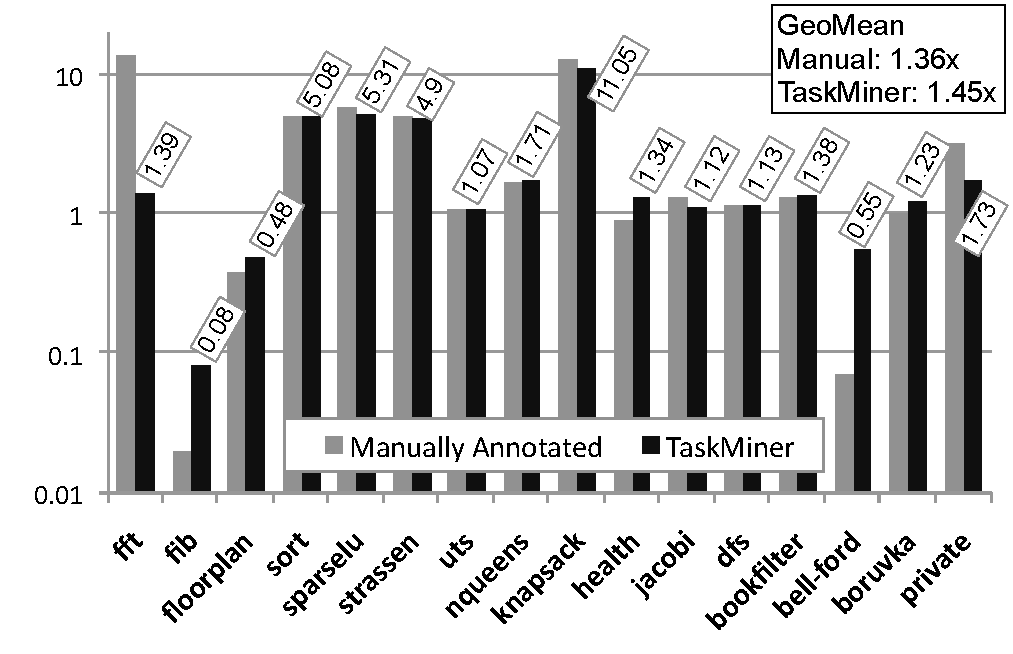
\includegraphics[width=1\columnwidth]{images/TM_Performance}
\caption{Comparações de performance. Anotações automáticas comparam-se favoralmente a intervenções
manuais, e levam à ganhos de desempenho. O eixo Y mostra o ganho de desempenho de cada versão anotada
pelo {\Taskminer} sobre a versão anotada manualmente. Os números nas pequenas caixas representam
o crescimento em velocidade obtido pelo {\Taskminer}.}
\label{fig:TM_Performance}
\end{center}
\end{figure}

A Figura~\ref{fig:TM_Performance} compara o tempo de execução de programas produzidos
pelo {\Taskminer} contra versões originais dos mesmos programas anotados manualmente.
Os {\em benchmarks} utilizados neste experimento são do \textsf{BSC-Bots}~\cite{Duran09} (\textsf{fft} até \textsf{jacobi}
na Fig.~\ref{fig:TM_Performance}) e do \textsf{Swan}~\cite{Moreira17}
(\textsf{dfs} até \textsf{private}).
Ambos vem com versões sequenciais e paralelas (anotadas manualmente). Os códigos foram compilados
com gcc-6.

As versões anotadas pelo \Taskminer{} foram mais velozes que as sequenciais em 13 dos 16 programas.
A maioria são algoritmos Dividir \& Conquistar clássicos como multiplicação de matrizes de \textsf{Strassen},
 \textsf{knapsack} (Problema da Mochila) e \textsf{fft}. Em 6 deles, as versões automáticas foram próximas e até
levemente acima das versões anotadas manualmente. Em 3 exemplos \Taskminer{} produziu versões piores que
as versões sequenciais: \textsf{fib}, \textsf{floorplan} e \textsf{bell-ford}. Entretanto, ainda assim produziu versões
mais rápidas que as anotadas manualmente. Uma inspeção visual de \textsf{bell-ford} indica que a versão
paralelizada manualmente dispara um número grande tarefas pequenas. O modelo de custo
do \Taskminer{} poda a criação de tarefas pequenas, mas não o suficiente para vencer o desempenho
da versão sequencial. Este experimento demonstra que \Taskminer{} pode trazer
ganhos consideráveis se comparados às versões sequenciais e manualmente anotadas.

%OPTIMIZATIONS
%Here, we show the results on two big optimizations: recursion depth and cost model.
%We can use the same benchmarks as above.
\subsection{Otimizações}
\label{sub:optimizations}

\begin{figure}[b!]
\begin{center}
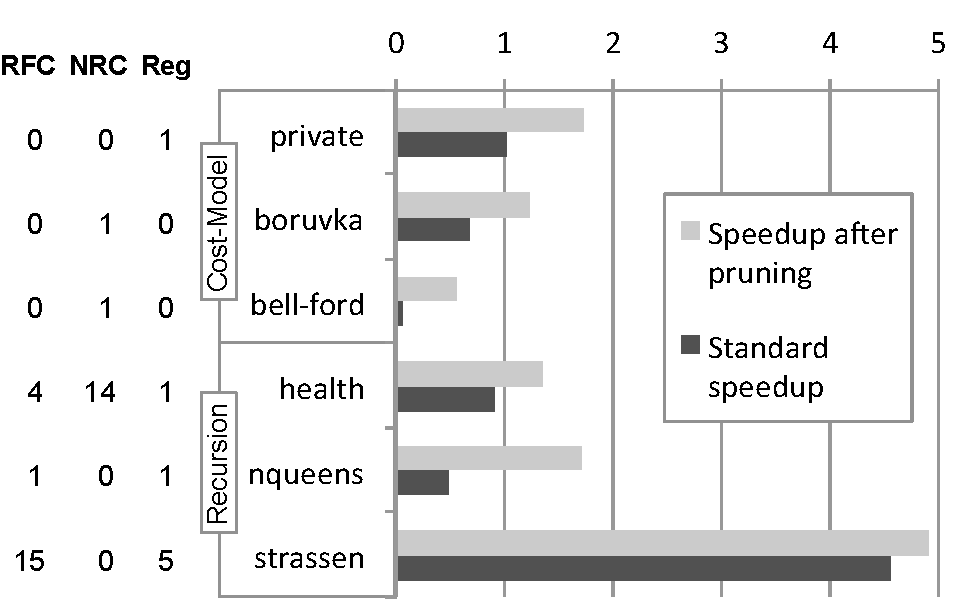
\includegraphics[width=1\columnwidth]{images/Optimizations}
\caption{Benefícios de limitar a criação de tarefas. (Secs.~\ref{sub:profit} e ~\ref{sub:ir}).
\textbf{CFR}: tarefas criadas em \underline{C}hamadas de \underline{F}unções \underline{R}ecursivas.
\textbf{CNR}: tarefas interprocedurais criadas ao redor de \underline{C}hamadas  \underline{N}ão-\underline{R}ecursivas.
\textbf{Reg}: tarefas envolvendo \underline{Reg}iões, sem chamadas de função.}
\label{fig:Optimizations}
\end{center}
\end{figure}

Este artigo descreve duas formas de otimizar a criação de tarefas. Ambas são baseadas na ideia de 
``poda de tarefas": evita-se a criação de tarefas consideradas não-lucrativas. A primeira técnica
corta criação de tarefas ditas não lucrativas de acordo com o modelo de custo, conforme explicado na 
Seção~\ref{sub:profit}; a segunda técnica corta criação de tarefas muito profundas na pilha de recursão, 
como descrito na Seção~\ref{sub:ir}. A Figura~\ref{fig:Optimizations} ilustra os benefícios dessas duas técnicas,
presentes em 6 dos benchmarks vistos anteriormente na Figura~\ref{fig:TM_Performance}.

Em 3 benchmarks, \textsf{private}, \textsf{boruvka} e
\textsf{bellman-ford}, o modelo de custo evita a criação de tarefas em laços que inicializam estruturas de dados.
Por exemplo, o laço a seguir, na linha 75 do programa \textsf{bellmanford.c}, seria paralelizado pelo
\Taskminer{}, caso o modelo de custo o marcasse como lucrativo:

\begin{verbatim}
  for (long unsigned i = 0; i < N; i++)
    for (long unsigned j = 0; j < N; j++)
      *(G + i * N + j) = rand();
\end{verbatim}

Similarmente, a limitação de tarefas recursivas (Sec.~\ref{sub:ir}), embora simples,
é efetiva em eliminar o excesso de tarefas pequenas. A Figura~\ref{fig:Optimizations} mostra o efeito
dessa otimização em três programas: \textsf{health}, \textsf{nqueens} e
\textsf{strassen}. Estes programas foram projetados para ilustrar paralelismo
em paradigma Dividir \& Conquistar ~\cite{Duran09}, e contém um grande número de chamadas
recursivas. A poda em níveis mais altos da árvore de recursão leva a ganhos de desempenho consideráveis
nestes programas. Caso não houvesse essa otimização de poda, então perda de desempenho seria observada
em  \textsf{health} e \textsf{nqueens}. Este experimento prova que as otimizações são efetivas
para melhorar a qualidade do código gerado pelo \Taskminer{}.

%VERSATILITY
%The goal here is to show that TaskMiner is a versatile tool, capable of finding many types of task parallelism in the code. 
%And the types of tasks that are going to be mined can be easily set, should the programmer ever desires to.
\subsection{Versatilidade}
\label{sub:versatility}

Os benchmarks das seções anteriores foram projetados especialmente para o estudo de 
paralelismo irregular. Para determinar se o \Taskminer{} consegue encontrar paralelismo 
em programas comuns, executou-se o mesmo sobre 219 programas escritos em C disponíveis
na suíte de testes do LLVM, e comparou-se o desempenho da versão anotada automaticamente pelo
\Taskminer{} com a versão original sequencial. 
\Taskminer{} anota um programa se:
(i) consegue encontrar limites simbólicos para todos os acessos à memória que ocorrem em uma hélice; e
(ii) a hélice é ampla o suficiente para pagar pelo custo de criação de tarefas no ambiente de execução.
Sob essas circunstâncias, descobriu-se tarefas em 63 desses programas. A Figura~\ref{fig:TM_Versatility} relaciona
o número de tarefas ao número de instruções em 30 dos maiores programas utilizados.
Para evitar a contagem de múltiplos arquivos C para o mesmo benchmark, a Figura~\ref{fig:TM_Versatility} contém
somente benchmarks que consistem em arquivos {\em single-source}. Como demonstrado neste experimento,
\Taskminer{} é capaz de anotar um número não trivial de benchmarks reais.

\begin{figure}[htb]
\begin{center}
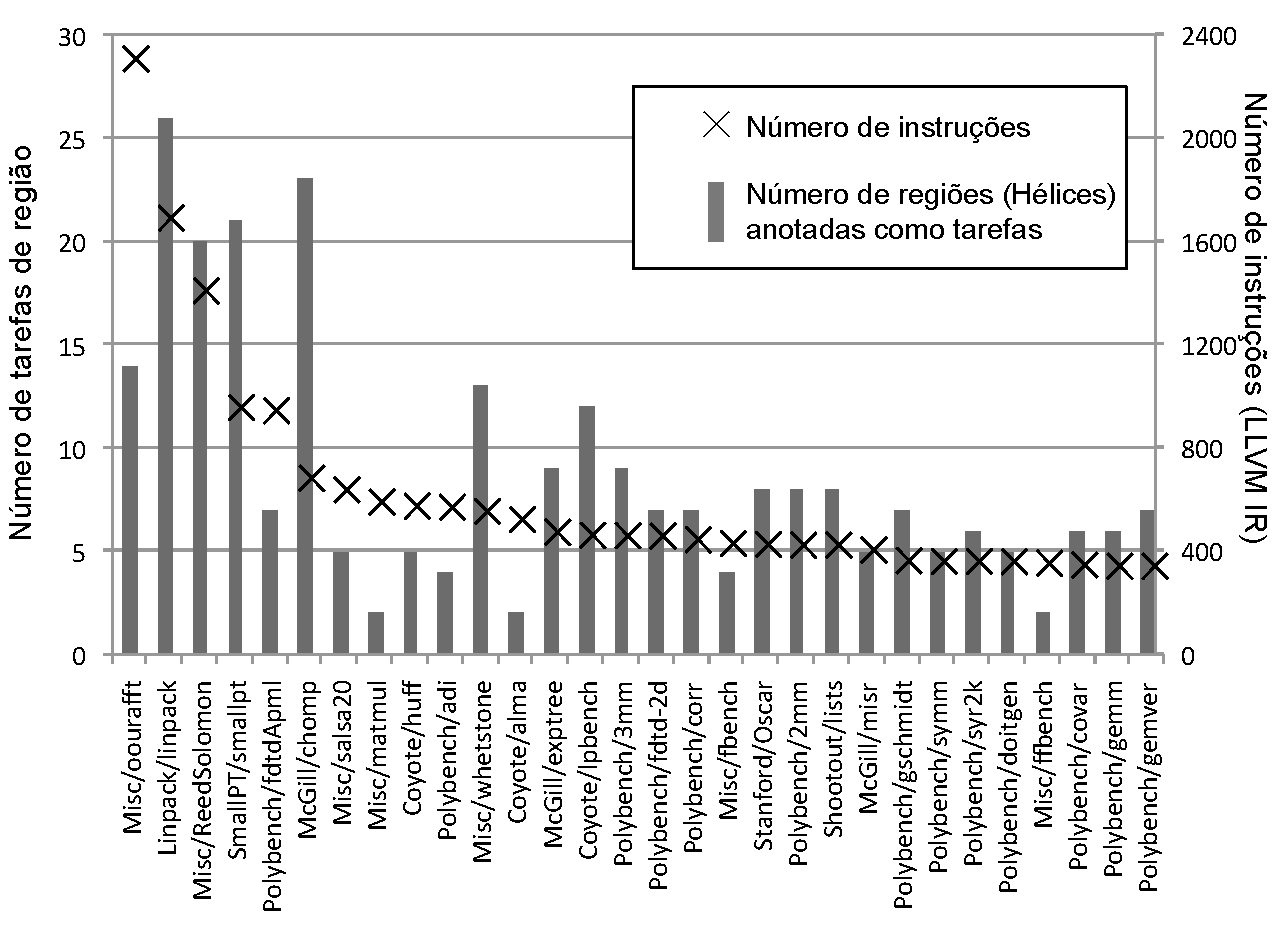
\includegraphics[width=1\columnwidth]{images/TM_Versatility}
\caption{Relação entre o número de regiões de tarefas e tamanho do programa.
Cada programa é um arquivo C completo.}
\label{fig:TM_Versatility}
\end{center}
\end{figure}

Observa-se que 27 dos benchmarks anotados não demonstraram aumento de desempenho em 
relação à versão sequencial,
pois as tarefas anotadas eram demasiadamente pequenas e pouco influenciaram na execução total do programa.
Em 17 benchmarks, observou-se uma perda de velocidade: neste caso, interações entre estruturas de dados
forçaram ao ambiente de execução do OpenMP a serizalizar a execução das tarefas. Essas perdas foram 
inferiores à 10\%. Em um dos casos, \textsf{MiBench/office-stringsearch}, a versão paralela foi 11 vezes mais lenta.
Por outro lado, obteve-se aumento de desempenho acima de 5\% em 19 benchmarks. 
Em \textsf{Misc/lowercase}, o acréscimo de velocidade foi acima de 3.5x, e em 3 casos, acima de 1.5x.
A Figura~\ref{fig:TM_GeneralProgs} mostra os 10 maiores acréscimos de desempenho obtidos pelo \Taskminer{}.
É importante enfatizar que esse experimento {\em não contou com nenhum tipo de intervenção humana}.
Portanto, \Taskminer{} é capaz de encontrar paralelismo automaticamente sem custo de programação.

\begin{figure}[t!]
\begin{center}
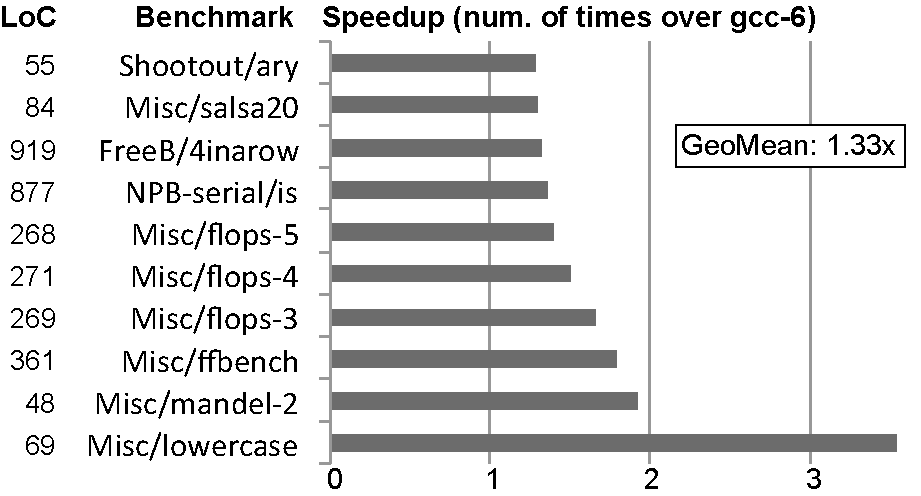
\includegraphics[width=1\columnwidth]{images/TM_GeneralProgs}
\caption{Melhorias de desempenho obtidas pelo \Taskminer{} quando aplicado à suíte de testes
do LLVM. Quanto maior a barra, maior o ganho de desempenho.
\textbf{LoC} significa ``Linhas de Código".}
\label{fig:TM_GeneralProgs}
\end{center}
\end{figure}


%{\Taskminer}'s versatility also arises in regards to the diversity of types of task parallelism that it
%can find in a program. Table \ref{tab:types} shows all types of tasks found in our main benchmarks.
%There are 3 types of tasks: recursive, which arises from vanes in Divide and Conquer
%algorithms; function call, which arises within loops that are not clearly parallel; and region, which 
%are similar to function calls, but instead are entire fragments of code within loops that can be executed in
%parallel. We provide the user complete decision power to mine for any type of tasks they wish when
%running our tool. 

%SCALABILITY
\subsection{Escalabilidade}
\label{sub:scalability}

\begin{figure}[htb]
\begin{center}
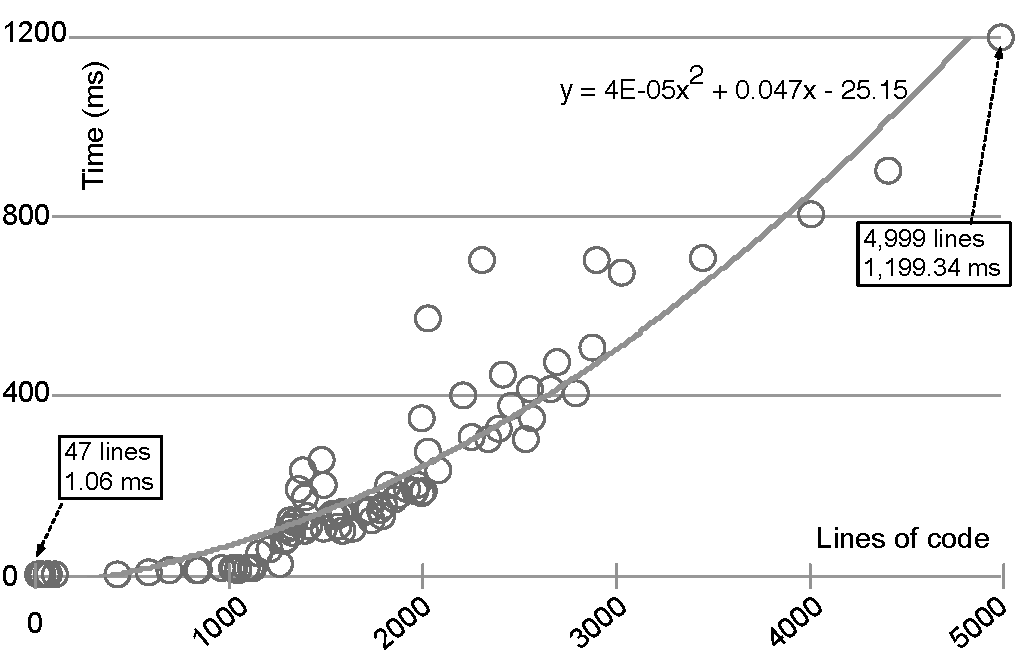
\includegraphics[width=0.9\columnwidth]{images/TM_Runtime}
\caption{Tempo de execução do \Taskminer{} versus tamanho dos programas.
Cada ponto representa um dos 100 programas gerados pelo \textsf{CSmith}.
A curva é uma aproximação polinomial de grau 2. O tamanho máximo obtido 
nos programas gerados pelo CSmith foi de 5.000 LoC.}
\label{fig:TM_Runtime}
\end{center}
\end{figure}

As análises descritas neste artigo possuem complexidade de tempo quadrática no pior caso.
Para testar a complexidade do algoritmo implementado na ferramenta \Taskminer{}, 
utilizou-se \textsf{CSmith}~\cite{Yang11}, um gerador de código aleatório, para produzir 
100 programas de tamanhos variados, os quais foram alimentados ao \Taskminer{}. 
A Figura~\ref{fig:TM_Runtime} mostra o resultado desse experimento.
O maior programa obtido teve 4.999 linhas de código, as quais foram processadas
pelo \Taskminer{} em 1.2 segundos.

\section{Trabalhos Relacionados}
\label{sec:rw}

Compiladores modernos adicionaram suporte ao paralelismo de tarefas do OpenMP apenas recentemente. Uma implementação
do compilador \textsf{clang} com esse suporte foi lançado em Março de 2014, por exemplo. Uma vez que a infra-estrutura necessária para
a implementação de tarefas é nova, não existem ferramentas além do {\Taskminer} capazes de anotar programas
automaticamente com essas diretivas.
Padrões de anotação baseados em diretivas provém aos programadores um modelo de programação paralela prático e fácil. Exemplos
de modelos que permitem paralelismo de tarefas são OpenMP 4.X,
StarSs \cite{bellens:sc:2006, perez:iccc:2008, planas:hpca:2009,
tejedor:hpdc:2011} e OmpSs \cite{bueno:icpp:2011, duran:ppl:2011}.
Por exemplo, Tareador \cite{Ayguade15} apresenta uma interface gráfica para identificação de potencial paralelismo e anotação de código sequencial.
Ao contrário do Tareador, {\Taskminer} executa essa tarefa automaticamente.

A técnica utilizada pelo {\Taskminer} para identificação de tarefas se assemelha às análises usadas durante
geração de código para máquinas de fluxo de dados. Programação de fluxo de dados foi originalmente proposta 
para facilitar paralelismo de tarefas~\cite{agrawal:ipdps:2010, chan:spaa:2007,
gupta:micro:2011}. Agrawal et al. \cite{agrawal:ipdps:2010} estendeu esse modelo
com inputs e outpus em Cilk++, que foi extendido novamente por ~\cite{vandierendonck:hotpar:2011} 
com cláusulas de dependência para facilitar
o projeto de padrões complexos de paralelsimo. Ambos apresentaram um escalonador unificado
baseado em paralelismo \textit{fork-join} \cite{vandierendonck:pact:2011} que permitiu
a execução de aplicações baseadas em tarefas. Outras abordagens também utilizaram grafos
de fluxo de dados para explorar paralelismo, como Tarefas Movidas à Dados \cite{tasirlar:icpp:2011},
em que o programador pode manipular cláusulas para determinar os argumentos da tarefa
antes de sua execução. Paralelismo baseado em função também foi proposto em \cite{gupta:micro:2011}
para utilizar argumentos de funções como especificadores de dependências entre tarefas.
Entretanto, a mineração e inserção automática dessas diretivas não consta como objetivo
em nenhum desses trabalhos.

Muitos sistemas foram desenvolvidos para extrair paralelismo de tarefas a partir de código sequencial.
Exemplos incluem OSCAR, Multigrain Parallelizing
Compiler \cite{ishizaka:journal:2000, kasahara:iwlcpc:2000},  MAPS \cite{castrillon:tii:2013, ceng:dac:2008}, e
DiscoPoP \cite{discopop, li:jss:2016}. Ferramentas como Paraver \cite{extrae, paraver},
Aftermath~\cite{drebes:hipeac:2014}, DAGvis \cite{huynh:wvpa:2015}, e TEMANEJO
\cite{brinkmann:parco:2011, brinkmann:journal:2013, temanejo} foram implementadas para 
permitir análise de desempenho e visualização de programas baseados em tarefas.
Apesar de ajudar o programar a adaptar o código paralelo, essas ferramentas não são 
inteiramente automáticas como o {\Taskminer}.


\section{Conclus\~{a}o}
\label{sec:conc}


\bibliography{references}

\end{document}
